\documentclass[a4paper, 11pt]{article} % Font size (can be 10pt, 11pt or 12pt) and paper size (remove a4paper for US letter paper)
\usepackage[utf8]{inputenc}
\usepackage[protrusion=true,expansion=true]{microtype} % Better typography
\usepackage{graphicx} % Required for including pictures
\usepackage{wrapfig} % Allows in-line images

\usepackage{mathpazo} % Use the Palatino font
\usepackage[T1]{fontenc} % Required for accented characters
\linespread{1.05} % Change line spacing here, Palatino benefits from a slight increase by default

\makeatletter
\renewcommand\@biblabel[1]{\textbf{#1.}} % Change the square brackets for each bibliography item from '[1]' to '1.'
\renewcommand{\@listI}{\itemsep=0pt} % Reduce the space between items in the itemize and enumerate environments and the bibliography

\renewcommand{\maketitle}{ % Customize the title - do not edit title and author name here, see the TITLE block below
\begin{flushright} % Right align
{\LARGE\@title} % Increase the font size of the title

\vspace{50pt} % Some vertical space between the title and author name

{\large\@author} % Author name
\\\@date % Date

\vspace{40pt} % Some vertical space between the author block and abstract
\end{flushright}
}

%----------------------------------------------------------------------------------------
%	TITLE
%----------------------------------------------------------------------------------------
\title{\textbf{MINERÍA DE DATOS}\\ % Title
Curso introductorio} % Subtitle

\author{\textsc{David Alejandro Trejo Pizzo} % Author
\\{\textit{-}}} % Institution

\date{\today} % Date
%----------------------------------------------------------------------------------------

\begin{document}

\maketitle
%----------------------------------------------------------------------------------------
%	ABSTRACT AND KEYWORDS
%----------------------------------------------------------------------------------------
%\renewcommand{\abstractname}{Summary} % Uncomment to change the name of the abstract to something else

\begin{abstract}
La minería de datos o exploración de datos (es la etapa de análisis de "Knowledge Discovery in Databases" o KDD) es un campo de las ciencias de la computación referido al proceso que intenta descubrir patrones en grandes volúmenes de conjuntos de datos. Utiliza los métodos de la inteligencia artificial, aprendizaje automático, estadística y sistemas de bases de datos. El objetivo general del proceso de minería de datos consiste en extraer información de un conjunto de datos y transformarla en una estructura comprensible para su uso posterior. Además de la etapa de análisis en bruto, que involucra aspectos de bases de datos y de gestión de datos, de procesamiento de datos, del modelo y de las consideraciones de inferencia, de métricas de Intereses, de consideraciones de la Teoría de la complejidad computacional, de post-procesamiento de las estructuras descubiertas, de la visualización y de la actualización en línea.
\end{abstract}

\hspace*{3,6mm}\textit{Keywords:} mineria de datos, algoritmos

\vspace{30pt}

%----------------------------------------------------------------------------------------
%	ESSAY BODY
%----------------------------------------------------------------------------------------

\section*{Introducción}

La minería de datos usa principios estadísticos contrastados para detectar patrones en los datos, ayudándole a tomar decisiones inteligentes sobre problemas complejos. La aplicación de los algoritmos de minería de datos de \textbf{Weka} a los datos le permitirá predecir tendencias, identificar patrones, crear reglas y recomendaciones, analizar la secuencia de eventos en conjuntos de datos complejos y obtener nuevos puntos de vista.\\

La minería de datos es el proceso de detectar la información procesable de los conjuntos grandes de datos. Utiliza el análisis matemático para deducir los patrones y tendencias que existen en los datos. Normalmente, estos patrones no se pueden detectar mediante la exploración tradicional de los datos porque las relaciones son demasiado complejas o porque hay demasiado datos.\\

Estos patrones y tendencias se pueden recopilar y definir como un modelo de minería de datos. Los modelos de minería de datos se pueden aplicar en escenarios como los siguientes:

\begin{itemize}
\item \textbf{Pronóstico:} cálculo de las ventas y predicción de las cargas del servidor o del tiempo de inactividad del servidor.
\item \textbf{Riesgo y probabilidad:} elección de los mejores clientes para la distribución de correo directo, determinación del punto de equilibrio probable para los escenarios de riesgo, y asignación de probabilidades a diagnósticos y otros resultados.
\item \textbf{Recomendaciones:} determinación de los productos que se pueden vender juntos y generación de recomendaciones.
\item \textbf{Búsqueda de secuencias:} análisis de los artículos que los clientes han introducido en la lista de compras y predicción de posibles eventos.
\item \textbf{Agrupación:} distribución de clientes o eventos en grupos de elementos relacionados, y análisis y predicción de afinidades.
\end{itemize}

\section*{Generación de modelos}

La generación de un modelo de minería de datos forma parte de un proceso mayor que incluye desde la formulación de preguntas acerca de los datos y la creación de un modelo para responderlas, hasta la implementación del modelo en un entorno de trabajo. Este proceso se puede definir mediante los seis pasos básicos siguientes:

\begin{enumerate}
\item Definir el problema
\item Preparar los datos
\item Explorar los datos
\item Generar modelos
\item Explorar y validar los modelos
\item Implementar y actualizar los modelos
\end{enumerate}

El siguiente diagrama describe las relaciones existentes entre cada paso del proceso:

\begin{center}
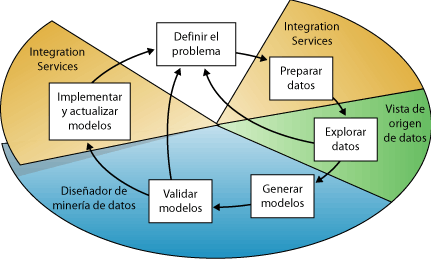
\includegraphics[width=300pt]{proceso}
\end{center}

El proceso que se ilustra en el diagrama es cíclico, lo que significa que la creación de un modelo de minería de datos es un proceso dinámico e iterativo. Una vez que ha explorado los datos, puede que descubra que resultan insuficientes para crear los modelos de minería de datos adecuados y que, por tanto, debe buscar más datos. O bien, puede generar varios modelos y descubrir entonces que no responden adecuadamente al problema planteado cuando los definió y que, por tanto, debe volver a definir el problema. Es posible que deba actualizar los modelos una vez implementados debido a que haya más datos disponibles. Puede que haya que repetir cada paso del proceso muchas veces para crear un modelo adecuado.

\subsection*{Definir el problema}

El primer paso del proceso de minería de datos, tal como se resalta en el siguiente diagrama, consiste en definir claramente el problema y considerar formas de usar los datos para proporcionar una respuesta para el mismo.\\

Este paso incluye analizar los requisitos empresariales, definir el ámbito del problema, definir las métricas por las que se evaluará el modelo y definir los objetivos concretos del proyecto de minería de datos. Estas tareas se traducen en preguntas como las siguientes:

\begin{itemize}
\item ¿Qué está buscando? ¿Qué tipos de relaciones intenta buscar?
\item ¿Refleja el problema que está intentando resolver las directivas o procesos de la empresa?
\item ¿Desea realizar predicciones a partir del modelo de minería de datos o solamente buscar asociaciones y patrones interesantes?
\item ¿Qué resultado o atributo desea predecir?
\item ¿Qué tipo de datos tiene y qué tipo de información hay en cada columna? En caso de que haya varias tablas, ¿cómo se relacionan? ¿Necesita limpiar, agregar o procesar los datos antes de poder usarlos?
\item ¿Cómo se distribuyen los datos? ¿Los datos son estacionales? ¿Los datos representan con precisión los procesos de la empresa?
\end{itemize}

Para responder a estas preguntas, puede que deba dirigir un estudio de disponibilidad de datos para investigar las necesidades de los usuarios de la empresa con respecto a los datos disponibles. Si los datos no abarcan las necesidades de los usuarios, podría tener que volver a definir el proyecto.\\

También debe considerar las maneras en las que los resultados del modelo se pueden incorporar en los indicadores de rendimiento clave (KPI) que se utilizan para medir el progreso comercial.

\section*{Preparar los datos}

El segundo paso del proceso de minería de datos, como se indica en el siguiente diagrama, consiste en consolidar y limpiar los datos identificados en el paso Definir el problema.\\

Los datos pueden estar dispersos en la empresa y almacenados en formatos distintos; también pueden contener incoherencias como entradas que faltan o incorrectas. Por ejemplo, los datos pueden mostrar que un cliente adquirió un producto incluso antes que se ofreciera en el mercado o que el cliente compra regularmente en una tienda situada a 2.000 kilómetros de su casa.\\

La limpieza de datos no solamente implica quitar los datos no válidos o interpolar valores que faltan, sino también buscar las correlaciones ocultas en los datos, identificar los orígenes de datos que son más precisos y determinar qué columnas son las más adecuadas para el análisis. Por ejemplo, ¿debería utilizar la fecha de envío o la fecha de pedido? ¿Qué influye más en las ventas: la cantidad, el precio total o un precio con descuento? Los datos incompletos, los datos incorrectos y las entradas que parecen independientes, pero que de hecho están estrechamente correlacionadas, pueden influir en los resultados del modelo de maneras que no espera.\\

Por consiguiente, antes de empezar a generar los modelos de minería de datos, debería identificar estos problemas y determinar cómo los corregirá. En la minería de datos, por lo general se trabaja con un conjunto de datos de gran tamaño y no se puede examinar la calidad de los datos de cada transacción; por tanto, es posible que necesite usar herramientas de generación de perfiles de datos, y de limpieza y filtrado automático de datos.

\subsection*{Explorar los datos}

El tercer paso del proceso de minería de datos, como se resalta en el siguiente diagrama, consiste en explorar los datos preparados.\\

Debe conocer los datos para tomar las decisiones adecuadas al crear los modelos de minería de datos. Entre las técnicas de exploración se incluyen calcular los valores mínimos y máximos, calcular la media y las desviaciones estándar, y examinar la distribución de los datos. Por ejemplo, al revisar el máximo, el mínimo y los valores de la media se podría determinar que los datos no son representativos de los clientes o procesos de negocio, y que por consiguiente debe obtener más datos equilibrados o revisar las suposiciones que son la base de sus expectativas. Las desviaciones estándar y otros valores de distribución pueden proporcionar información útil sobre la estabilidad y exactitud de los resultados. Una desviación estándar grande puede indicar que agregar más datos podría ayudarle a mejorar el modelo. Los datos que se desvían mucho de una distribución estándar se podrían sesgar o podrían representar una imagen precisa de un problema de la vida real, pero dificultan el ajustar un modelo a los datos.\\

Al explorar los datos para conocer el problema empresarial, puede decidir si el conjunto de datos contiene datos defectuosos y, a continuación, puede inventar una estrategia para corregir los problemas u obtener una descripción más profunda de los comportamientos que son típicos de su negocio.

\subsection*{Generar modelos}

El cuarto paso del proceso de minería de datos, como se resalta en el siguiente diagrama, consiste en generar el modelo o modelos de minería de datos. Usará los conocimientos adquiridos en el paso Explorar los datos para definir y crear los modelos.\\

Deberá definir qué columnas de datos desea que se usen; para ello, creará una estructura de minería de datos. La estructura de minería de datos se vincula al origen de datos, pero en realidad no contiene ningún dato hasta que se procesa. Al procesar la estructura de minería de datos, \textbf{Weka} genera agregados y otra información estadística que se puede usar para el análisis. Cualquier modelo de minería de datos que esté basado en la estructura puede utilizar esta información.\\

Antes de procesar la estructura y el modelo, un modelo de minería de datos simplemente es un contenedor que especifica las columnas que se usan para la entrada, el atributo que está prediciendo y parámetros que indican al algoritmo cómo procesar los datos. El procesamiento de un modelo a menudo se denomina entrenamiento. El entrenamiento hace referencia al proceso de aplicar un algoritmo matemático concreto a los datos de la estructura para extraer patrones. Los patrones que encuentre en el proceso de entrenamiento dependerán de la selección de los datos de entrenamiento, el algoritmo que elija y cómo se haya configurado el algoritmo.\\

También puede utilizar los parámetros para ajustar cada algoritmo y puede aplicar filtros a los datos de entrenamiento para utilizar un subconjunto de los datos, creando resultados diferentes. Después de pasar los datos a través del modelo, el objeto de modelo de minería de datos contiene los resúmenes y modelos que se pueden consultar o utilizar para la predicción.\\

\subsection*{Validar modelos}

El quinto paso del proceso de minería de datos, como se resalta en el siguiente diagrama, consiste en explorar los modelos de minería de datos que ha generado y comprobar su eficacia.\\

Antes de implementar un modelo en un entorno de producción, es aconsejable probar si funciona correctamente. Además, al generar un modelo, normalmente se crean varios con configuraciones diferentes y se prueban todos para ver cuál ofrece los resultados mejores para su problema y sus datos.\\

\textbf{Weka} proporciona herramientas que ayudan a separar los datos en conjuntos de datos de entrenamiento y pruebas, para que pueda evaluar con precisión el rendimiento de todos los modelos en los mismos datos. El conjunto de datos de entrenamiento se utiliza para generar el modelo y el conjunto de datos de prueba para comprobar la precisión del modelo mediante la creación de consultas de predicción. 

\subsection*{Actualizar modelos}

El último paso del proceso de minería de datos, como se resalta en el siguiente diagrama, consiste en implementar los modelos que funcionan mejor en un entorno de producción.\\

Una vez que los modelos de minería de datos se encuentran en el entorno de producción, puede llevar acabo diferentes tareas, dependiendo de sus necesidades. Las siguientes son algunas de las tareas que puede realizar:

\begin{itemize}
\item Use los modelos para crear predicciones que luego podrá usar para tomar decisiones comerciales.
\item Crear consultas de contenido para recuperar estadísticas, reglas o fórmulas del modelo.
\item Incrustar la funcionalidad de minería de datos directamente en una aplicación. 
\item Actualizar los modelos después de la revisión y análisis.
\item Actualizar dinámicamente los modelos, cuando entren más datos en la organización, y realizar modificaciones constantes para mejorar la efectividad de la solución debería ser parte de la estrategia de implementación.
\end{itemize}


\section*{Algoritmos de minería de datos}

Un algoritmo de minería de datos es un conjunto de cálculos y reglas heurísticas que permite crear un modelo de minería de datos a partir de los datos. Para crear un modelo, el algoritmo analiza primero los datos proporcionados, en busca de tipos específicos de patrones o tendencias. El algoritmo usa los resultados de este análisis para definir los parámetros óptimos para la creación del modelo de minería de datos. A continuación, estos parámetros se aplican en todo el conjunto de datos para extraer patrones procesables y estadísticas detalladas.\\

El modelo de minería de datos que crea un algoritmo a partir de los datos puede tomar diversas formas, incluyendo:

\begin{itemize}
\item Un conjunto de clústeres que describe cómo se relacionan los casos de un conjunto de datos.
\item Un árbol de decisión que predice un resultado y que describe cómo afectan a este los distintos criterios.
\item Un modelo matemático que predice las ventas.
\item Un conjunto de reglas que describen cómo se agrupan los productos en una transacción, y las probabilidades de que dichos productos se adquieran juntos.
\end{itemize}

\subsection*{Tipos de algoritmos}

La elección del mejor algoritmo para una tarea analítica específica puede ser un desafío. Aunque puede usar diferentes algoritmos para realizar la misma tarea, cada uno de ellos genera un resultado diferente, y algunos pueden generar más de un tipo de resultado. Por ejemplo, puede usar el algoritmo Árboles de decisión no solo para la predicción, sino también como una forma de reducir el número de columnas de un conjunto de datos, ya que el árbol de decisión puede identificar las columnas que no afectan al modelo de minería de datos final.\\

Tipos de algoritmos:
\begin{itemize}
\item Algoritmos de clasificación, que predicen una o más variables discretas, basándose en otros atributos del conjunto de datos.
\item Algoritmos de regresión, que predicen una o más variables continuas, como las pérdidas o los beneficios, basándose en otros atributos del conjunto de datos.
\item Algoritmos de segmentación, que dividen los datos en grupos, o clústeres, de elementos que tienen propiedades similares.
\item Algoritmos de asociación, que buscan correlaciones entre diferentes atributos de un conjunto de datos. La aplicación más común de esta clase de algoritmo es la creación de reglas de asociación, que pueden usarse en un análisis de la cesta de compra.
\item Algoritmos de análisis de secuencias, que resumen secuencias o episodios frecuentes en los datos, como un flujo de rutas web.
\end{itemize}

\subsection*{Estructuras de minería de datos}

La estructura de minería de datos define los datos a partir de los cuales se generan los modelos de minería de datos: especifica la vista de datos de origen, el número y el tipo de columnas, y una partición opcional en conjuntos de entrenamiento y de pruebas. Una misma estructura de minería de datos puede admitir varios modelos de minería de datos que comparten el mismo dominio. En el diagrama siguiente, se muestra la relación de la estructura de minería de datos con el origen de datos y con los modelos de minería de datos que la componen.

\begin{center}
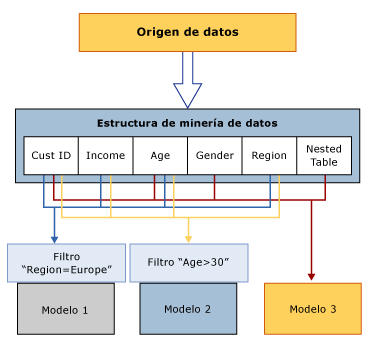
\includegraphics[width=300pt]{estructura}
\end{center}

La configuración de una estructura de minería de datos consta de los pasos siguientes:

\begin{itemize}
\item Definir un origen de datos.
\item Seleccionar las columnas de datos que se van a incluir en la estructura (no es necesario agregar todas las columnas al modelo) y definir una clave.
\item Definir una clave para la estructura, incluyendo la clave de la tabla anidada, si procede.
\item Especificar si los datos de origen se deben separar en un conjunto de entrenamiento y en un conjunto de prueba. Este paso es opcional.
\item Procesar la estructura.
\end{itemize}

Cuando se define una estructura de minería de datos, se usan columnas que están disponibles en una vista del origen de datos existente. Una vista del origen de datos es un objeto compartido que permite combinar varios orígenes de datos y usarlos como un origen único. Los orígenes de datos originales no son visibles para las aplicaciones cliente, y puede usar las propiedades de la vista del origen de datos para modificar tipos de datos, crear agregaciones o asignar alias a las columnas.\\

Si genera varios modelos de minería de datos a partir de la misma estructura de minería de datos, los modelos pueden usar columnas diferentes de la estructura. Por ejemplo, puede crear una estructura única y, a continuación, generar modelos independientes de árbol de decisiones o de agrupación en clústeres a partir de ella, donde cada uno de ellos pueda usar columnas diferentes y predecir atributos distintos.

\section*{Modelos}

Un modelo de minería de datos se crea mediante la aplicación de un algoritmo a los datos, pero es algo más que un algoritmo o un contenedor de metadatos: es un conjunto de datos, estadísticas y patrones que se pueden aplicar a los nuevos datos para generar predicciones y deducir relaciones.\\

En esta sección se explica qué es un modelo de minería de datos y cuál puede ser su uso: la arquitectura básica de modelos y estructuras, las propiedades de los modelos de minería de datos y las maneras de crear modelos de minería de datos y trabajar con ellos.\\

Un modelo de minería de datos recibe los datos de una estructura de minería de datos y, a continuación, los analiza utilizando un algoritmo de minería de datos. La estructura y el modelo de minería de datos son objetos independientes. La estructura de minería de datos almacena la información que define el origen de datos. Un modelo de minería de datos almacena la información derivada del procesamiento estadístico de los datos, como los patrones encontrados como resultado del análisis.\\

Un modelo de minería de datos está vacío hasta que los datos que proporciona la estructura de minería de datos se procesan y analizan. Una vez procesado el modelo, contiene los metadatos, resultados y enlaces de la estructura de minería de datos.\\

Los metadatos especifican el nombre del modelo y el servidor donde está almacenado, así como una definición del mismo, incluidas las columnas de la estructura de minería de datos que se usaron para generarlo, las definiciones de los filtros que se aplicaron al procesarlo y el algoritmo empleado para analizar los datos. Todas estas opciones, las columnas de datos y sus tipos de datos, filtros y algoritmo, influyen en gran medida en los resultados del análisis.\\

Por ejemplo, puede usar los mismos datos para crear varios modelos, quizás mediante un algoritmo de clústeres, un algoritmo de árboles de decisión y un algoritmo Bayes Naïve. Cada tipo de modelo crea un conjunto diferente de patrones, conjuntos de elementos, reglas o fórmulas, que puede usar para realizar predicciones. Por lo general, cada algoritmo analiza los datos de forma diferente, por lo que el contenido del modelo resultante también se organiza en estructuras diferentes. En un tipo de modelo, los datos y los modelos pueden estar agrupados en clústeres; en otro, los datos pueden estar organizados en árboles, ramas y las reglas que los dividen y definen.\\

El modelo también se ve afectado por los datos usados en el entrenamiento: incluso los modelos cuyo entrenamiento se ha realizado en la misma estructura de minería de datos pueden producir resultados distintos si se filtran los datos de manera diferente o se usan semillas distintas durante el análisis. Sin embargo, los datos reales no se almacenan en el modelo; solo lo hacen las estadísticas de resumen, mientras que los datos reales residen en la estructura de minería de datos. Si ha creado filtros en los datos al realizar el entrenamiento del modelo, las definiciones de filtro también se guardan con el objeto de modelo.\\

El modelo contiene un conjunto de enlaces, que señalan a los datos almacenados en memoria caché en la estructura de minería de datos. Si los datos se han almacenado en memoria caché en la estructura y no se han borrado después del procesamiento, estos enlaces le permiten obtener detalles de los resultados para llegar a los casos en que se basan los resultados. Sin embargo, los datos reales están almacenados en la memoria caché de la estructura, no en el modelo.\\

Para crear un modelo de minería de datos, siga estos pasos generales:

\begin{itemize}
\item Cree la estructura de minería de datos subyacente e incluya las columnas de datos que sean necesarias.
\item Seleccione el algoritmo más adecuado para la tarea analítica.
\item Elija las columnas de la estructura que se incluirán en el modelo y especifique cómo se deben usar, es decir, qué columna contiene el resultado que desea predecir, qué columnas son únicamente para la entrada, etc.
\item \textbf{Opcionalmente}, puede establecer los parámetros para ajustar el procesamiento del algoritmo.
\item Rellene el modelo con datos procesando la estructura y el modelo.
\end{itemize}

\section*{Prueba y validación}

La validación es el proceso de evaluar cuál sería el rendimiento de sus modelos de minería de datos con datos reales. Es importante que valide sus modelos de minería de datos entendiendo su calidad y sus características antes de implementarlos en un entorno de producción.\\

Existen muchos enfoques a la hora de evaluar la calidad y las características de un modelo de minería de datos.

\begin{itemize}
\item Use varias medidas de validez estadística para determinar si existen problemas en los datos o en el modelo.
\item Separe los datos en conjuntos de entrenamiento y de prueba con el fin de probar la precisión de predicciones.
\item Solicite a los expertos comerciales que revisen los resultados del modelo de minería de datos para determinar si los patrones detectados tienen sentido en un escenario empresarial concreto.
\end{itemize}

Todos estos métodos son útiles para la metodología de minería de datos y se usan de forma iterativa a la hora de crear, probar y refinar modelos para responder a un problema concreto. No hay ninguna regla completa única que pueda indicarle si un modelo es suficientemente bueno, o si cuenta con suficientes datos.

\subsection*{Criterios para validar modelos}

Las medidas de minería de datos se suelen agrupar en las categorías de precisión, confiabilidad y utilidad.\\

La \textbf{precisión} es una medida que indica hasta qué punto el modelo pone en correlación un resultado con los atributos de los datos que se han proporcionado. Existen varias medidas de precisión, pero todas ellas dependen de los datos que se utilicen. En realidad, podrían faltar valores o éstos ser aproximados, o incluso diferentes procesos podrían cambiar los datos. En particular, en la fase de exploración y desarrollo, podría decidir aceptar una cierta cantidad de errores en los datos, sobre todo si éstos son suficientemente uniformes en sus características. Por ejemplo, un modelo que predice las ventas para un almacén determinado en base a las ventas pasadas puede estar muy correlacionado y ser muy preciso, incluso si ese almacén ha utilizado un método de contabilidad equivocado continuamente. Por tanto, es necesario equilibrar las mediciones de precisión mediante las valoraciones de confiabilidad.\\

La \textbf{confiabilidad} evalúa la manera en la que se comporta un modelo de minería de datos en conjuntos de datos diferentes. Un modelo de minería de datos es confiable si genera el mismo tipo de predicciones o encuentra los mismos tipos generales de patrones independientemente de los datos de prueba que se proporcionen. Por ejemplo, el modelo que ha generado para el almacén que utilizó un método de contabilidad equivocado no podría extrapolarse correctamente a otros almacenes, y por tanto, no sería confiable.\\

La \textbf{utilidad} incluye diferentes métricas que le indican si el modelo proporciona información útil. Por ejemplo, un modelo de minería de datos que pone en correlación la ubicación del almacén con las ventas podría ser preciso y fiable, pero podría no ser útil, ya que no se podría generalizar ese resultado si se agregaran más almacenes en la misma ubicación. Es más, no responde a la pregunta comercial fundamental de porqué ciertas ubicaciones tienen más ventas que otras. También podría descubrir que un modelo que parece correcto, en realidad no tiene sentido porque está basado en correlaciones cruzadas de los datos.

\end{document}